\documentclass[pdftex,12pt,letter]{article}
\usepackage{fancyhdr}
\usepackage{enumerate}
\usepackage{tabularx}
\usepackage{graphicx}
\usepackage{array}
\usepackage[justification=justified,singlelinecheck=false]{caption}
\usepackage{placeins}
\pagestyle{fancy}
\makeatletter
  \renewcommand\@seccntformat[1]{\csname the#1\endcsname.\quad}
\makeatother

\newcolumntype {Y}{ >{\raggedright \arraybackslash }X}
\newcommand{\HRule}{\rule{\linewidth}{0.5mm}}
\captionsetup{labelformat=empty}

\begin{document}

\begin{titlepage}
\begin{flushright}
\HRule \\[0.4cm]
{ \bfseries
{\huge Design Document\\[1cm]}
{\Large for\\[1cm]}
{\huge CWRUtility\large\\[4cm]}
{\large Prepared by\\Jason Kuster, Stuart Long, and William Ordiway\\[1cm]
Version 1.0 \\[1cm]
KOALAA Development\\[1cm]
October 10, 2012}}
\end{flushright}
\end{titlepage}
\tableofcontents{}
\begin{table}[!t]
\caption*{\bfseries Revision History}
\begin{tabularx}{\textwidth }[t]{|l|Y|Y|l|}
\hline
\bfseries Name & \bfseries Date & \bfseries Reasons for Change & \bfseries Version \\ \hline
Long & 10/6/2012 & Initial Outline & 1.0 initial\\
Kuster, Long, Ordiway & 10/10/12 & Initial Draft & 1.0\\
\hline
\end{tabularx}
\end{table}
\FloatBarrier
\newpage
\clearpage
\section{Overview}
\subsection{Overall Design}
The \emph{CWRUtility} application is essentially a collection of CWRU-related features that allows for easy, centralized access to each of the features. The complete list of features and their description can be found in the \emph{CWRUtility} SRS. Since this software system can be easily broken down into separate, uncoupled features, the design of the overall system is also broken down. Each feature will have it's own design, documented below in the "Features" section, that will operate independently of the other features. The only exception to this rule is the "StartPage" feature, which can also be seen as the overall application manager. Explained in detail below, the "StartPage" feature will be responsible for navigating the system to the different features and controlling any communication between the features. \textbf{Figure~\ref{fig:overall}} below
shows the various components of the system and how they are linked. This
diagram could be seen as the highest level of design for the system. \textbf{Figure~\ref{fig:sequence}} shows the sequence diagram for the same system. Every page in the application is represented by a XAML file and a C\# "behind" file that handles
the actual functionality.
\begin{figure}[h!]
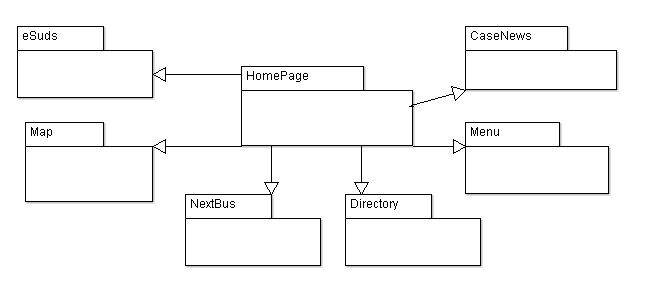
\includegraphics[width=120mm]{OverallCD.png}
\caption{\textbf{Figure~\ref{fig:overall}} Package Diagram}
\label{fig:overall}
\end{figure}
\begin{figure}[h!]
\includegraphics[width=120mm]{sequenceDia.png}
\caption{\textbf{Figure~\ref{fig:sequence}} Sequence Diagram}
\label{fig:sequence}
\end{figure}
\FloatBarrier
\subsection{User Interface}
The implementation of any user interfaces on the Windows Phone 7/8 platform is done using the eXtensible Application Markup Language (XAML). Essentially, XAML can be used as a layout language similar to HTML. XAML provides a straightforward way to generate, lay out, and populate the on-screen elements. Data population will be done by using Model View View-Model (MVVM), a data-binding interface built into the Windows Phone SDK. The data fields will be laid out in XAML, which will comprise the view; the code to map the data to the view is contained in the view-model, and the raw data will be stored in application storage.It is important to note that a markup language is very dissimilar to a programming language as it works through simply creating a series of attributes and assigning values to them. The Windows Phone OS actually handles creating the UI based on these attributes, therefore this software system does not have to. 
\\
\section{Features}
\subsection{StartPage}
The "StartPage" feature represents both the manager for the rest of the application and the feature the user is taken to on application start-up. This feature actually comprises two different application pages for the "At-a-glance" page and one for the page listing the full list of features.
\subsubsection{Class Diagram}
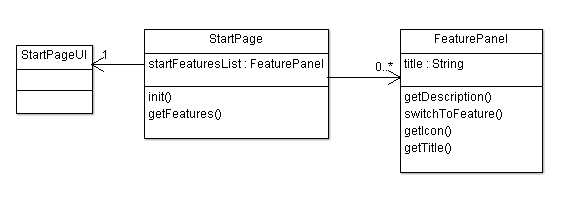
\includegraphics[width=120mm]{StartPageCD.png}
\subsubsection{StartPage}
The StartPage class will be the main class in this feature. It will be the feature that opens when the user starts the application, an operation that is handled by the XAML (UI) file. The page will display the application title at the top, then the feature title below that, and finally a scrollable list of featurePanels. Each featurePanel will represent one of the other features within the application and will display the feature title as well as a potentially "live" description for that feature. For example, one of the features in this feature panel will be the "nextBus" feature, and its feature panel will display the next shuttle time for the user's last selected stop. This page will display all of the applications features in a scrollable list. If the user clicks on a feature panel, the application will switch the user to that feature.
\subsubsection{FeaturePanel}
There will be an instance of feature panel for every feature in the application. A featurePanel will store the title of the feature and a description for that feature. Since descriptions can be "live", or constantly updating its information, some of the instances of featurePanel will have to override the getDescription() method in order to properly display the correct up-to-date information. The "StartPage" class will send a list of these FeaturePanels to the UI manager so that they can be displayed to the user. The switchToFeature() will be called when the user selects a featurePanel from the displayed list. The application then creates a new instance of the selected feature and switches to that feature.
\subsubsection{UIManager}
The XAML file responsible for laying out the components of this feature for display to the user. This feature will have the title of the application and then the title of this feature. Under the titles, the majority of the feature will be taken up by a scrollable list of featurePanels. The XAML file will get the list of featurePanels by calling the getFeatures() method in the StartPage class. 
\subsection{Map}
The "Map" feature will allow the users to view a two maps of the Case Western Reserve University Campus. The first map will be a road map displayed using the interactive map controller provided by the Windows Phone SDK. This map controller is the same map controller used for the default Windows Phone 7 map application. Since the map controller is already provided by the Windows Phone SDK, the implementation of this portion of the feature is straightforward. The application will also add MapLayers to the map to portray CWRU specific information to the user, such as an outline of the campus and push pins for the major landmarks on campus. The other map the feature will display will be the official campus map of the university.  This map will be loaded into the application as an image and any desired manipulation of the iamge will have to be coded in directy because the map controller cannot be used with any map other than the default Bing map.
\subsubsection{Class Diagram}
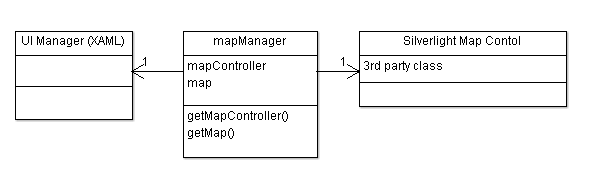
\includegraphics[width=120mm]{MapCD.png}
\subsubsection{SilverlightMapControl}
The SilverlightMapControl class is part of a third party library provided by Microsoft Corporation. It provides basic map controls such as zooming in, zooming out, and panning for any provided map. The map control API is in control of the RoadMode class that is extended by CWRUMapMode.
\subsubsection{CWRUMapMode}
The CWRUMapMode class extends the RoadMode class \\(Microsoft.Phone.Controls.Maps.RoadMode). The CWRUMapMode class is responsible for limiting the map control provided bing map to just displaying the CWRU campus. validLats and validLongs are the ranges for the latitudes and the longitudes that the user should be able to view on the map, ie the latitudes and longitudes for CWRU's campus. getZoomRange() should be called by constrainView() and it restrict what level of zoom the user is allowed to zoom into and outto when viewing the map. constrainView() is a class from RoadMode that gets called every time a user interacts with the map. CWRUMapMode will have to override the class to ensure the user stays within the valid latitude/longitude ranges.
\subsubsection{MapManager}
The MapManager class is responsible for handling the other two classes: the SilverlightMapControl and the UI manager. The MapManager will create the map object, actualMap, and sets its mode to a new instance of the CWRUMapMode. Furthermore, the MapManager will create the additional map layers. The map layers will include an outline of campus, created using a MapPolyline object, and PushPin objects designating major landmarks on campus.  It will also be responsible for sending the SilverlightMapControl to the UI manager so that the UI manager can display the map. The toggleLayerButton\_Click method will be used for handling user's requests to hide or show the current map layer.\\\\While the XAML file will be responsible for uploading and displaying the official CWRU map to the user as an image. Manipulation on the image will have to be handled by the behind MapManager class, thus necessitating the handleZoom method.
\subsubsection{XAML File}
This file will be responsible for laying out the components of the feature. Since two different maps will be represented, each map will gets it own semi page within the feature, known as "pivots". Users can swipe laterally on the phone to switch between the two maps. This display schematic can be completely handled within the XAML file. For each map, it will layout the title of the application at the top, the name of this feature below that, and the actual maps will take up most of the application. The XAML file will be sent the map controller (along with that map controller's view, i.e. the map) by the MapManager. The XAML file will also load the official CWRU map as an image and will query the MapManager upon user interaction in order to appropriately manipulate the image.
%william's section
\subsection{Directory}
The "Directory" feature will allow users to view the location, hours, phone number, and a description of the wide assortment of Case Western Reserve University campus resources. This feature consists of a list of resources names that are expandable to reveal information about that resource. The operation of this feature is simple to grasp: a text file which containing information for all campus resources in read and converted into a string, parsed and converted into multiple resources which are added to a list in the Directory class and then list is presentend in the windows phone friendly format with the help of readFromFile() operation.
\subsubsection{Class Diagram}
\begin{flushleft}
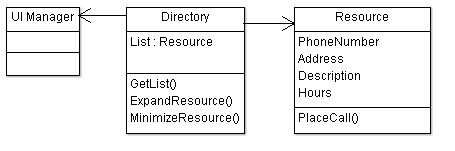
\includegraphics[width=120mm]{DirectoryCD.png}
\end{flushleft}
\subsubsection{Resource}
Each campus resource that will be represented in our application will be represented as an object in the resource class possessing a Phone Number, an Address, open hours, and a brief description about what the resource can be used for. The address, open hours, and description will all be simple text variables which are displayed on screen. However the phone number variable is tied to the PlaceCall() operation. By tapping the phone number of a resource the user’s phone will place a call to that number. This information about every campus resource will be manually loaded into the app by the developers and in the event that a resource was omitted or a new resource is offered by the campus this feature will have to be updated to include that resource. 
\subsubsection{Directory}
The directory class is used to maintain a variable List which contains a number of resource objects, each of which represent a different campus resource. Selecting a campus resource by touching it on the screen with your finger will expand information about that resource with the ExpandResource() operation and shut the previous, if any, selected resource with a MinimizeResource() operation. Every time a resource is expanded the LastOpened resource (if any) is minimized and then LastOpened points to the newly opened resource so if a new resource is opened this one will be shut. This keeps the list managable to scroll through, since expanding a resource reveals multiple lines of information and so if every resource were aloud to be expanded at the same time there would be exponentially more data for a user to scroll through on his/her search for a resource. Selecting an already open resource will also minimize it.
\subsubsection{XAML}
The XAML file will display the application title, followed by this feature title
(Directory), and then the names of resources which can be tapped to display relative information. The list of resources can be navigated by scrolling up or down with swipes of the finger. 
\subsection{NextBus}
The "NextBus" feature will allow the users to interface with the NextBus, Inc. bus times prediction website. This feature will offer users the ability to select bus routes, bus direction, and stops in order to facilitate the use of the "Greenie" bus system on campus. The feature's main page will be a single Windows Phone-style page with three drop-down selection boxes and a "Go" button. There will be a field, initially blank, which will populate with the next prediction times (max 3). Additionally, the NextBus section will feature on the main page, where it will provide a small icon which contains the stop which the user has marked as "default".
\subsubsection{Class Diagram}
\begin{flushleft}
\includegraphics[width=120mm]{nextbusCD.png}
\end{flushleft}
\subsubsection{BusScheduleManager}
The BusScheduleManager class handles retrieval and formatting of the NextBus data. Since Case Western has not purchased the feed option from NextBus, aggregating data will require scraping the HTML that NextBus generates for each bus stop once it is requested. This class will also handle the drop-down menus, populating them with the requisite items once route and direction have been selected. There are two listener methods which will populate the next dropdown in the list when the previous item is successfully selected. Additionally, there is a method which runs when the "Go" button is pressed, which will pull the requisite info from the NextBus website and display it on the screen.
\subsubsection{UIManager}
The UIManager for this feature will not be a true class, since all UI for Windows Phone is done using XAML files. Still, this manager will be responsible for laying out the components of the feature. Namely, it will have to lay out the title of the application at the top, and the name of this feature below that. There will be three dropdown menus on the top of the screen - one for Route, Direction, and Stop. There will be a "Go" button underneath which will initiate the prediction request. There will be a "set default" button, which will set the bus that is loaded on the main page, as well as the one to which the NextBus page will default on load. Additionally, there will be three text boxes, initially empty, which will populate once the predictions are acquired.
\subsection{eSuds}
The eSuds feature will allow the users to interface with the eSuds laundry interface. This feature offers users the ability to query the eSuds service for the statuses of the washers and driers in the buildings on campus, and provides visual feedback on the status of the individual machines - red for in progress, green for free. This will be presented in a table-formatted list box containing all of the machines and their states. There will be a small part of the main menu devoted to eSuds and it will list the building set as default, as well as the number of free washers and dryers.
\subsubsection{Class Diagram}
\begin{flushleft}
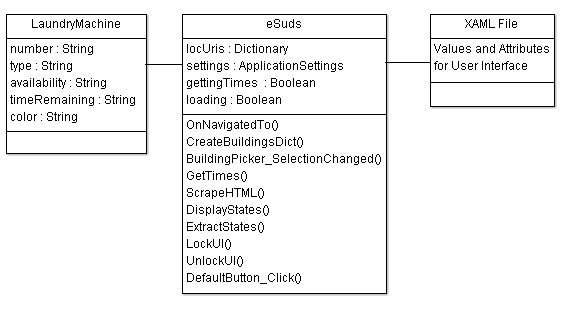
\includegraphics[width=120mm]{eSuds.png}
\end{flushleft}
\subsubsection{eSudsManager}
The eSudsManager class is in charge of retrieval and formatting of eSuds data. Similarly to NextBus, eSuds does not have a publicly accessible API. Thus, we will be scraping the data from their website and formatting it for viewing on a phone screen instead of a web browser. As there is only one menu, there will be no go button because the act of clicking on a building is sufficient input. There is one listener method waiting for this action.
\subsubsection{LaundryMachine}
As there is a decent amount of metadata relating to a laundry machine, it was necessary to create a class to describe them. The LaundryMachine class contains a number of elements, each with a getter and setter. The elements are:
\begin{enumerate}
\item Number: The laundry machine's number, displayed on its front.
\item Type: Denotes whether the machine is a washer or dryer.
\item Availability: Can be one of four states: Available, In Use, Cycle Complete, or Unavailable.
\item timeRemaining: If the machine is currently "In Use", it will have an estimated time to completion.
\item color: Contains the color this machine should be displayed as - green for "Available", red for anything else.
\end{enumerate}
\subsubsection{UIManager}
The UIManager for this feature will not be a true class, since all UI for Windows Phone is done using XAML files. Still, this manager will be responsible for laying out the components of the feature. Namely, it will have to lay out the title of the application at the top, and the name of this feature below that. There will be one dropdown menu which will allow for building selection, and a table with a column for each LaundryMachine attribute except for color, and a row for each LaundryMachine object which it is handed. The status for each LaundryMachine will have its color set to the "color" attribute.
%\subsection{Schedule}
%The "Schedule" feature will allow users to add classes or custom events to a saved schedule on the system. This feature will require three classes: a schedule event, a schedule event manager to handle schedule events, and a UI manager for the schedule.
\subsection{Case News}
The "Case News" feature will display the prominent new stories from the
two main sources of CWRU news: \emph{The Case Daily} and \emph{The Observer}. The
stories will be displayed in a list format with a panel per story containing the
stories' headline. If a user clicks on a particular story that story will expand
to display the story in its entirety. Both news sources have RSS feed so this
class will simply act as a RSS reader for those two feeds.
\subsubsection{Class Diagram}
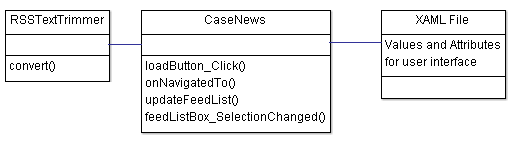
\includegraphics[width=120mm]{CaseNewsCD.png}
\subsubsection{CaseNews}
This class is the main class for this feature. It will be responsible for querying the Daily and the Observer for news stories and passing them to the
XAML file to be displayed (this communication will done through data binding). This class will also check news stories should be refreshed (on user
request) and will consequently refresh the stories. There will be a refresh
button displayed, whose action is handled by loadButton\_click which calls
update\_feedList. onNavigated To will build the list for the first time a user
switches to this feature.
\subsubsection{RSSTextTrimmer}
The RSSTextTrimmer takes in raw RSSText feed from an RSS feed and
trims for output onto a Windows Phone 7/8 display. This conversion is handled in the convert method. The conversion performs actions like removing
unnecessary whitespace and html tags from the input.
\subsubsection{XAML File}
The XAML file will display the application title, followed by this feature title
(Case News), and then a list of the stories from the two news sources. It will
get the titles and descriptions of the stories from the CaseNews class through
data binding.
\lfoot{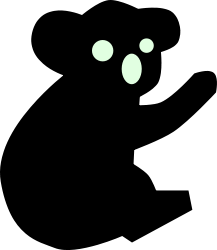
\includegraphics[height=1cm]{DarkKoala.png}}

%\subsection{Class Diagram}
%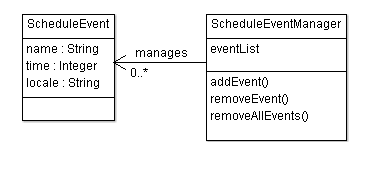
\includegraphics[width=80mm]{ScheduleEventsCD.png}
%\figurename{Schedule Class Diagram}
%\subsection{Class Descriptions}
%The following class descriptions describe the above class diagram.
%\subsubsection{ScheduleEvent}



\subsection{Menus}
The Menus feature displays menus for the campus' major dining halls (Fribley Marche and Leutner Cafe). The system will display one menu at a time, allowing application users to select which location they would like to look by selecting a dinning hall's name at the top of the feature page or by swiping horizontally across the screen. Additionally the user can select what day's menu to view up to the end of the week. Bon Appetit, Case Western's dining service, offers and RSS feed so the data to support this feature will be gathered through that.
\subsubsection{Class Diagram}
\begin{flushleft}
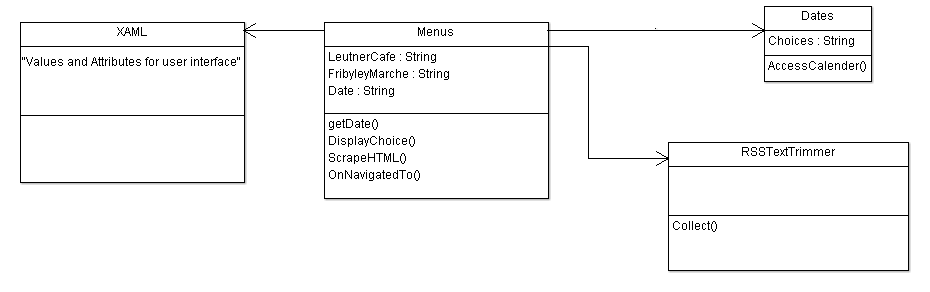
\includegraphics[width=120mm]{MenuCD.png}
\end{flushleft}
\subsubsection{MenusClass}
This class utilizes the RSSTextTrimmer class to populate and maintains two strings which store all of the dinning selections, one for each dinning hall and so the strings are named Fribley and Leutner. The getDate() operation gets the current date from the phone and uses that to select what menus will be displayed by default if the user of the application does not specify a date they want to observe the menu for. The user can select a different date by clicking a dropdown at the bottom of the screen which activates Menus OnNavigatedTo() operation which directs to a new page generated by the Dates class listing every day for the week, upon tapping a date the user is returned to the original Menus feature page and presented with the menu of Fribley or Leutner for that day.
\subsubsection{RSSTextTrimmer}
The RSSTextTrimmer takes in raw RSSText feed from an RSS feed and
puts the gathered data into the Fribley and Leutner strings which are parsed and manipulated by the DisplayChoice() method in the Menu class which optimizes the data for Windows Phone 7/8 display. The conversion performs actions like removing
unnecessary whitespace and html tags from the input. Additionally only the menu for the relevant date (the current date, unless the user has specified a different date) and the relevant dining hall.
\subsubsection{Dates}
The dates class can access the calender on the Windows Phone to populate a string called Choices with the days of the current week. The Present() operation displays this string in such a manner that each day is selectable and updates the date variable in the Menus class.
\subsubsection{XAML}
The XAML file will display the application title, followed by this feature title
(Menus), and then the names 'Fribley' and 'Leutner' which can be tapped to display the respective menus. Alternative the menu not currently being viewed can be accessed by swiping a finger across the screen as well. At the bottom of the screen is a dropdown menu which, if selected, brings the user to a new page where they may select a day in the current week. After their selection they are brought back to the original menu's page and presented with the menu for the day of their choice.



\end{document}
